%Use one of the two documentclass lines depending on aspect ratio needed
% for 4x3 aspect ratio slides
%\documentclass{beamer}
%for 16x9 (modern wide screen) aspect ratio slides
\documentclass[aspectratio=169]{beamer}

% Oxford Maths theming
\usetheme{oxfordmaths}
\usepackage{tikz}
\usepackage{appendixnumberbeamer}
\usepackage{booktabs}
\usepackage{ragged2e}
\usepackage{xcolor}
\usetikzlibrary{positioning, arrows.meta, shapes.geometric}
\usetikzlibrary{decorations.pathreplacing}
\usetikzlibrary{positioning, arrows.meta}
\usetikzlibrary{arrows.meta,calc} 
% \definecolor{oxfordblue}{RGB}{0,33,71}
% colours
\definecolor{softblue}{RGB}{232,238,246}
\definecolor{softpink}{RGB}{252,232,242}
\definecolor{softyellow}{RGB}{255,248,220}
\definecolor{softpurple}{RGB}{242,232,245}
\definecolor{softgreen}{RGB}{232,245,236}
\definecolor{softorange}{RGB}{255,239,222}
\definecolor{darkblue}{RGB}{0,33,71}
\definecolor{darkpink}{RGB}{155,65,105}
\definecolor{darkyellow}{RGB}{150,110,20}
\definecolor{darkpurple}{RGB}{95,55,120}
\definecolor{darkgreen}{RGB}{40,120,75}
\definecolor{darkorange}{RGB}{180,95,20}
\definecolor{RoadBlue}{RGB}{0,0,205}
\definecolor{RoadGreen}{RGB}{0,100,0}
\definecolor{RoadRed}{RGB}{200,0,0}



\usepackage[most]{tcolorbox}
\newtcolorbox{specbox}[2]{
    enhanced,
    colback=#1!5,
    colframe=#1!75!black,
    coltitle=white,
    colbacktitle=#1!75!black,
    title=#2,
    arc=2mm,
    boxrule=0pt,
    left=2mm,
    right=2mm,
    top=1mm,
    bottom=1mm,
    fonttitle=\bfseries
}

% Set author etc info
\title[Efficient Spectral Computations] %short version of title for slide footer
{Efficient Algorithms for Infinite-Dimensional Spectral Computations} %full title for titlepage
\author{Maggie McCarthy \\ Supervisor: Prof. Patrick Farrell}
\institute{Mathematical Institute\\University of Oxford}
\date[5 June 2026]  %short date for slide footer
% {Really Great Conference, May 2024} %main date for title page,
                        %can overload it to show say 'Conference X, Date Y'


%% Now for the actual slides %%
\begin{document}

\begin{frame}[plain]
  \titlepage
\end{frame}

\begin{frame}{The Spectra of Linear Operators}
  % \framesubtitle{A bit more information about this}

\begin{specbox}{blue}{Definition}
Consider a linear operator $A$ on a Hilbert space $H.$ The spectrum of $A$ is 
  $$ \text{Sp}(A) = \{ z \in \mathbb{C} \mid (A-zI)^{-1} \text{ does not exist as a bounded operator} \}.$$
\end{specbox}


  % Consider a linear operator $A$ on a Hilbert space $H.$ The spectrum of $A$ is 
  % \vspace{1em}
  % $$ \text{Sp}(A) = \{ z \in \mathbb{C} \mid (A-zI)^{-1} \text{ does not exist as a bounded operator} \}.$$


\vspace{1em}

 Computing $\text{Sp}(A)$ is a fundamental problem in mathematics with many applications.

 \vspace{0.5em}


  \begin{figure}
      \centering
      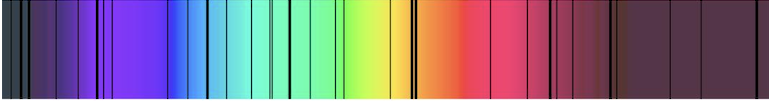
\includegraphics[width=1\linewidth]{spec_lines.png}
      \caption{\footnotesize The black `Fraunhofer lines' in a spectroscopic image of the sun's light correspond to the differences of eigenvalues of the Schrödinger operator for atoms such as H, Fe, Ca, Na, and Mg.}
      \label{fig:placeholder}
  \end{figure}

% Spectroscopic measurements such as these led to the discovery of the expanding universe.  
  
  
\end{frame}

\begin{frame}{$\operatorname{Sp}(A)$ in Finite and Infinite Dimensions}

\only<1->{
\begin{specbox}{blue}{Definition}
\[
\operatorname{Sp}(A)
=
\left\{
z\in\mathbb{C}
\,:\,
(A-zI)^{-1} \text{ does not exist as a bounded operator}
\right\}.
\]
\end{specbox}


\vspace{0.3em}

\begin{specbox}{green!45!black}{Finite dimensions}
In finite dimensions, $A$ is an $n\times n$ matrix and $\operatorname{Sp}(A)$ is the set of eigenvalues of $A,$ i.e.,
\[
\operatorname{Sp}(A)
=
\left\{
\lambda\in\mathbb{C}
\,:\,
Av=\lambda v \text{ for some } v\neq 0
\right\}.
\]
\end{specbox}
}

\only<2->{
\vspace{0.3em}

\begin{specbox}{red}{Infinite dimensions}
In infinite dimensions, $\operatorname{Sp}(A)$ may contain more than the eigenvalues of $A$.
It can have both discrete and continuous parts, making it much harder to compute.
\end{specbox}
}

\end{frame}


% \begin{frame}{$\text{Sp}(A)$ in Finite and Infinite Dimensions}

% \begin{tcolorbox}[
%     colback=green!5,
%     colframe=green!75!black,
%     coltitle=white,
%     colbacktitle=green!75!black,
%     title=Definition,
%     arc=2mm,
%     boxrule=0pt,
%     left=2mm,
%     right=2mm,
%     top=1mm,
%     bottom=1mm]

% $$ \text{Sp}(A) = \{ z \in \mathbb{C} \mid (A-zI)^{-1} \text{ does not exist as a bounded operator} \}.$$

% \end{tcolorbox}

% \vspace{0.3em}

% \begin{tcolorbox}[
%     colback=blue!5,
%     colframe=blue!70!black,
%     coltitle=white,
%     colbacktitle=blue!70!black,
%     title=Finite dimensions,
%     arc=2mm,
%     boxrule=0pt,
%     left=2mm,
%     right=2mm,
%     top=1mm,
%     bottom=1mm
% ]
% If $A$ is an $n\times n$ matrix, then $\text{Sp}(A)$ is the set of eigenvalues of $A:$
% \[
% \operatorname{Sp}(A)
% =
% \{\lambda\in\mathbb{C}: Av=\lambda v \text{ for some } v\neq 0\}.
% \]
% \end{tcolorbox}

% \vspace{0.3em}

% \begin{tcolorbox}[
%     colback=red!5,
%     colframe=red!75!black,
%     coltitle=white,
%     colbacktitle=red!75!black,
%     title=Infinite dimensions,
%     arc=2mm,
%     boxrule=0pt,
%     left=2mm,
%     right=2mm,
%     top=1mm,
%     bottom=1mm
% ]
% In infinite dimensions, $\text{Sp}(A)$ may contain more than the eigenvalues of $A.$ It may have both continuous and discrete parts, making it much harder to compute.
% \end{tcolorbox}
% \end{frame}

% \begin{frame}{Computing $\text{Sp}(A)$ in infinite dimensions}

% The standard approach in infinite dimensions is to discretize the problem, compute the spectra of the corresponding finite-dimensional operator, $A_h,$ and hope that the set of computed eigenvalues approaches $\text{Sp}(A).$ 
% \vspace{1em}
% $$
% A
% \;\xrightarrow{\text{discretize}}\;
% A_h
% \;\xrightarrow{\text{solve}}\;
% \operatorname{Sp}(A_h)
% \approx
% \operatorname{Sp}(A).
% $$
% \vspace{0.75em}

% To use the finite element methodology, we construct the variational formulation of $Au = zu$ in some infinite-dimensional space $V,$ project it into a finite-dimensional space $V_h,$ and solve the discretized problem for an approximation of $\text{Sp}(A).$

% \end{frame}

\begin{frame}{Infinite-Dimensional Spectra: An Example}

\only<1->{

\begin{specbox}{red}{Infinite dimensions}
In infinite dimensions, $\operatorname{Sp}(A)$ may contain more than the eigenvalues of $A$.
It can have both discrete and continuous parts, making it much harder to compute.
\end{specbox}


\vspace{0.6em}

\begin{columns}[T,onlytextwidth]
\begin{column}{0.62\textwidth}
% For example, consider the right shift operator on $\ell^2$:
% \[
% R(u_1,u_2,u_3,\ldots)=(0,u_1,u_2,u_3,\ldots).
% \]

% \vspace{0.5em}

% Its spectrum is the closed unit disk,
% \[
% \operatorname{Sp}(R)=\{z\in\mathbb{C}: |z|\leq 1\},
% \]
% but it has no eigenvalues.
\vspace{1em}
For example, the right shift operator defined in $\ell^2,$
$$ A(u_1, u_2, \dots) = (0, u_1, u_2, \dots),$$
has a spectrum equal to the closed unit disk, but it has no eigenvalues. 
\end{column}

\begin{column}{0.35\textwidth}
\centering
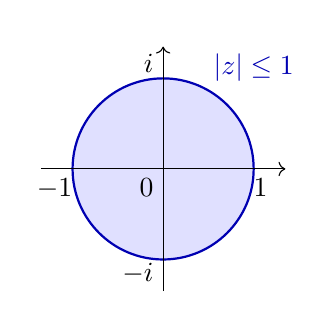
\begin{tikzpicture}[scale=1.15]
    % filled disk
    \fill[blue!12] (0,0) circle (1);
    \draw[thick,blue!70!black] (0,0) circle (1);

    % axes
    \draw[->] (-1.35,0) -- (1.35,0) node[right]{};
    \draw[->] (0,-1.35) -- (0,1.35) node[above]{};

    % point labels
    \node[below left] at (0,0) {$0$};
    \node[below,xshift=2.5pt] at (1,0) {$1$};
    \node[below,xshift=-6.5pt] at (-1,0) {$-1$};
    \node[left,yshift=5.5pt] at (0,1) {$i$};
    \node[left,yshift=-5pt] at (0,-1) {$-i$};

    % text inside upper-right part of disk
    \node[blue!70!black] at (1.0,1.12) {$|z|\leq 1$};
\end{tikzpicture}
\end{column}
\end{columns}
}

\end{frame}
\begin{frame}{Computing \(\operatorname{Sp}(A)\) in Infinite Dimensions}

\begin{columns}[T,onlytextwidth]

\begin{column}{0.60\textwidth}

The standard approach in infinite dimensions is to discretize $A$ with an $n$-dimensional operator, $A_n,$ and hope that $\text{Sp}(A_n)$ approaches $\text{Sp}(A).$

% to discretize the problem, compute the spectra of the corresponding finite-dimensional operator, $A_h,$ and hope that the set of computed eigenvalues approaches $\text{Sp}(A).$ 
% the problem with a finite-dimensional operator, $A_h,$ solve for $\text{Sp}(A_h),$ and hope that  $\text{Sp}(A_h),$
% \begin{itemize}
%     \item to discretize the problem 
%     \item compute the spectra of the corresponding finite-dimensional operator, $A_h,$ and
%     \item hope that the set of computed eigenvalues approaches $\text{Sp}(A).$
% \end{itemize}

\vspace{0.2cm}

\[
A
\;\xrightarrow{\text{discretize}}\;
A_n
\;\xrightarrow{\text{solve}}\;
\operatorname{Sp}(A_n)
\stackrel{?}{\approx}\;
\operatorname{Sp}(A).
\]
% \[
% A
% \;\xrightarrow{\text{discretize}}\;
% A_h
% \;\xrightarrow{\text{solve}}\;
% \operatorname{Sp}(A_h)
% \rightarrow \;
% \operatorname{Sp}(A) \text{ as } n \rightarrow \infty?
% \]

\vspace{0.3cm}

To use the finite element method, we
\begin{itemize}
    \item formulate the variational eigenproblem in an infinite-dimensional space \(V\),
    \item restrict the problem to a finite-dimensional space $V_n,$ and
    \item solve the discrete eigenproblem for $\text{Sp}(A_n).$
\end{itemize}

\vspace{0.2cm}

% In a basis, this gives a generalized matrix eigenproblem
% \[
% KU = \lambda_h MU.
% \]
\end{column}

\begin{column}{0.36\textwidth}
% \textbf{Reference}

% \vspace{0.2cm}

% \small
% D. Boffi,\\
% \emph{Finite Element Approximation of Eigenvalue Problems},\\
% Acta Numerica, 2010.

% \vspace{0.4cm}

% optional book/article image
\begin{center}
    
\includegraphics[width=0.75\linewidth]{daniele-boffi.jpg}

    \vspace{0.15cm}

    {\scriptsize
    \begin{minipage}{0.9\linewidth}
    \centering
    Reference: D. Boffi, \emph{Finite Element Approximation of Eigenvalue Problems}, Acta Numerica, 2010.
    \end{minipage}
    }
\end{center}
\end{column}

\end{columns}

\end{frame}

% \begin{frame}{How do we compute \(\operatorname{Sp}(A)\)?}

% In finite dimensions, \(A\) is an \(n\times n\) matrix and
% \[
% \operatorname{Sp}(A)=\{\lambda\in\mathbb{C}: Au=\lambda u
% \text{ for some }u\neq 0\}.
% \]

% \vspace{0.3cm}

% In infinite dimensions, \(\operatorname{Sp}(A)\) may contain more than eigenvalues:
% \[
% \text{point spectrum} \quad + \quad \text{continuous spectrum}.
% \]

% \vspace{0.3cm}

% The standard numerical approach is:

% \[
% A
% \quad \longrightarrow \quad
% A_h
% \quad \longrightarrow \quad
% \operatorname{Sp}(A_h)
% \approx
% \operatorname{Sp}(A).
% \]

% \vspace{0.3cm}

% For finite elements, choose \(V_h\subset V\), project the variational eigenproblem onto \(V_h\), and solve the resulting finite-dimensional eigenvalue problem.

% \end{frame}


% \begin{frame}{Dangerous pitfalls}

% \textbf{Spectral pollution:} The discretized operator has eigenvalues that converge to $z \notin \text{Sp}(A).$

% \vspace{1em}

% \textbf{Spectral invisibility:} discretizing the operator causes us to miss parts of its spectrum,
% even as the size of the discretization increases.

% \vspace{1em}

% \textbf{Failure to compute the essential spectrum:}  In infinite dimensions, $\text{Sp}(A)$ may contain continuous, or essential, components that are extremely difficult or impossible to compute in a finite-dimensional setting.

    
% \end{frame}

\begin{frame}{Dangerous Pitfalls of the Discretize-Then-Solve Approach}

    

\begin{columns}[T,onlytextwidth]

% ---------------- LEFT COLUMN ----------------
\begin{column}{0.48\textwidth}
\small

\textbf{Spectral pollution:}  
The discretized operator has eigenvalues that converge to $z \notin \text{Sp}(A).$

\vspace{2em}

\textbf{Spectral invisibility:}  
discretizing the operator causes us to miss parts of its spectrum,
even as the size of the discretization increases.


\vspace{2em}

\textbf{Failure to compute essential spectra:}  
In infinite dimensions, $\text{Sp}(A)$ may contain continuous or essential components that are extremely difficult or impossible to compute in a finite-dimensional setting.

\end{column}

% ---------------- RIGHT COLUMN ----------------
% \begin{column}{0.55\textwidth}
% \centering
% \resizebox{\linewidth}{!}{%
% \begin{tikzpicture}[x=1cm,y=1cm, every node/.style={font=\small}]
\begin{column}{0.49\textwidth}
\centering
\resizebox{!}{0.72\textheight}{%
    \begin{tikzpicture}[x=1cm,y=1cm, every node/.style={font=\small}]

% ---------- common dimensions ----------
\def\W{10.8}
\def\H{3.1}

% =========================================================
% 1. Spectral Pollution
% =========================================================
\begin{scope}[shift={(0,0)}]
    \draw[thick] (0,0) rectangle (\W,\H);

    \node[font=\bfseries] at (\W/2,2.7) {Spectral Pollution};

    \node at (\W/2,2.15) {\(\operatorname{Sp}(A)\)};
    \draw[decorate,decoration={brace,amplitude=5pt}] (1.7,1.7) -- (9.1,1.7);

    % true spectrum
    \draw[line width=0.8pt] (1.9,1.45) -- (4.6,1.45);
    \draw[line width=0.8pt] (5.8,1.45) -- (8.9,1.45);

    % computed spectrum
    \draw[dotted, line width=1.2pt] (1.8,0.9) -- (8.95,0.9);

    % spurious point
    \draw[gray] (5.15,0.9) circle (0.23);
    \fill (5.15,0.9) circle (0.08);

    \draw[->] (6.2,1.15) -- (5.4,0.97);
    \node at (7.4,1.15) {spurious limit};

    \node at (\W/2,0.25) {\(\operatorname{Sp}(A_h)\)};
    \draw[decorate,decoration={brace,mirror,amplitude=5pt}] (1.7,0.75) -- (9.1,0.75);
\end{scope}

% =========================================================
% 2. Spectral Invisibility
% =========================================================
\begin{scope}[shift={(0,-3.7)}]
    \draw[thick] (0,0) rectangle (\W,\H);

    \node[font=\bfseries] at (\W/2,2.7) {Spectral Invisibility};

    \node at (\W/2,2.15) {\(\operatorname{Sp}(A)\)};
    \draw[decorate,decoration={brace,amplitude=5pt}] (1.8,1.6) -- (9,1.6);

    % true spectrum
    \draw[line width=0.8pt] (1.9,1.45) -- (4.35,1.45);
    \draw[line width=0.8pt] (6.25,1.45) -- (8.65,1.45);

    % computed spectrum only sees one part
    \draw[dotted, line width=1.2pt] (6.25,1) -- (8.65,1);

    \draw[->] (3.1,1.1) -- (3.1,1.40);
    \node at (3.25,0.9) {missed spectrum};

    \node at (7.68,0.25) {\(\operatorname{Sp}(A_h)\)};
    \draw[decorate,decoration={brace,mirror,amplitude=5pt}] (6,0.8) -- (9,0.8);
\end{scope}

% =========================================================
% 3. Continuous and Essential Spectra
% =========================================================
\begin{scope}[shift={(0,-7.4)}]
    \draw[thick] (0,0) rectangle (\W,\H);

    \node[font=\bfseries] at (\W/2,2.7) {Continuous and Essential Spectra};

    \node[align=left] at (1.9,1.65) {discrete\\spectra};
    \fill (3.35,1.78) circle (0.06);
    \fill (3.70,1.45) circle (0.06);
    \fill (3.60,1.98) circle (0.06);

    \draw[line width=0.9pt] (3.55,0.5)
        .. controls (4.2,0.95) and (6.9,1.00) ..
        (7.7,1.70)
        .. controls (7.85,1.95) and (7.75,2.10) ..
        (7.82,2.35);

    \node[align=left] at (8.8,1.15) {continuous\\or essential\\spectra};
\end{scope}

\end{tikzpicture}%
}
\end{column}
\end{columns}

\end{frame}

\begin{frame}{An Example of Spectral Pollution: The Maxwell Eigenproblem}
Let $V = H_0(\operatorname{rot};U)$ and $U = (0, \pi)^2.$

\vspace{1em}

The variational formulation of the Maxwell eigenproblem is to find $\omega\in\mathbb R\setminus\{0\}$ and nonzero $\mathbf E \in V$ such that
% Let $V = H_0(\operatorname{rot};U)$ and $U = (0, \pi)^2.$ 
% \newline
% \textbf{Variational formulation:} Find $\omega\in\mathbb R\setminus\{0\}$ and a nonzero $\mathbf E \in V \text{ such that }$
% $$ \text{Find } \omega\in\mathbb R\setminus\{0\} \text{ and a nonzero } \mathbf E \in V \text{ such that }
$$\int_{U} \operatorname{rot}\mathbf E \,\, \overline{\operatorname{rot}\mathbf v} \, dx = \omega^2 \int_{U} \mathbf E \cdot \overline{\mathbf v} \, dx \qquad
\forall \mathbf v\in V.
$$

\vspace{1em}

The squares of the eigenvalues, $\omega^2,$ correspond to the Neumann eigenvalues of the Laplacian in $U.$ Thus,
$$ \omega^2 = n^2 + m^2 \qquad \text{for } n, m \in \mathbb{N}_0, \qquad (m,n) \ne (0, 0).$$ 
\end{frame}


\begin{frame}{An Example of Spectral Pollution: The Maxwell Eigenproblem}

\uncover<1->{
Using standard Lagrange continuous piecewise linear elements yields spectral pollution:
}

\only<2->{
\vspace{-0.6em}

{
\centering
\begingroup
\footnotesize
\setlength{\tabcolsep}{6pt}
\renewcommand{\arraystretch}{1.0}

\begin{tabular}{ccc|c}
\toprule
\uncover<2->{$N=4$}
&
\uncover<3->{$N=8$}
&
\uncover<4->{$N=16$}
&
\uncover<5->{$N=\infty$}
\\
\midrule

\uncover<2->{$-2.220446\cdot 10^{-16}$}
&
\uncover<3->{$2.220446\cdot 10^{-16}$}
&
\uncover<4->{$2.220446\cdot 10^{-16}$}
&
\uncover<5->{$0$}
\\

\uncover<2->{$\vdots$}
&
\uncover<3->{$\vdots$}
&
\uncover<4->{$\vdots$}
&
\uncover<5->{$\vdots$}
\\

\uncover<2->{$1.017010$}
&
\uncover<3->{$1.004276$}
&
\uncover<4->{$1.001070$}
&
\uncover<5->{$1$}
\\

\uncover<2->{$1.017010$}
&
\uncover<3->{$1.004276$}
&
\uncover<4->{$1.001070$}
&
\uncover<5->{$1$}
\\

\uncover<2->{$2.067822$}
&
\uncover<3->{$2.017113$}
&
\uncover<4->{$2.004283$}
&
\uncover<5->{$2$}
\\

\uncover<2->{$4.264703$}
&
\uncover<3->{$4.068039$}
&
\uncover<4->{$4.017105$}
&
\uncover<5->{$4$}
\\

\uncover<2->{$4.264703$}
&
\uncover<3->{$4.068039$}
&
\uncover<4->{$4.017105$}
&
\uncover<5->{$4$}
\\

\uncover<2->{$5.397073$}
&
\uncover<3->{$5.106342$}
&
\uncover<4->{$5.026739$}
&
\uncover<5->{$5$}
\\

\uncover<2->{$5.397073$}
&
\uncover<3->{$5.106342$}
&
\uncover<4->{$5.026739$}
&
\uncover<5->{$5$}
\\

\uncover<2->{\alt<6->{$\textcolor{red}{\mathbf{5.671192}}$}{$5.671192$}}
&
\uncover<3->{\alt<6->{$\textcolor{red}{\mathbf{5.922934}}$}{$5.922934$}}
&
\uncover<4->{\alt<6->{$\textcolor{red}{\mathbf{5.980743}}$}{$5.980743$}}
&
\uncover<5->{\alt<6->{$\textcolor{red}{\mathbf{6}}$}{$6$}}
\\

\bottomrule
\end{tabular}

\endgroup
\par
}
}

\uncover<6->{
\vspace{0.5em}

Whether spectral pollution occurs depends on the choice of mesh and finite elements.
}

\end{frame}


\begin{frame}{A Remedy for the Pitfalls}
    % A reliable algorithm for computing $\text{Sp}(A)$ should converge as the size of the discretization, $n,$ tends towards infinity and guarantee that any point of the output is close to $\text{Sp}(A),$ up to an arbitrary small error tolerance. 
    % \end{itemize}
    % \begin{itemize}
    %     \item  converge as the size of the discretization, $n,$ tends towards infinity.
    %     \item  guarantee that any point of the output is close to $\text{Sp}(A),$ up to an arbitrary small error tolerance. 
    % \end{itemize}

    \begin{columns}[T]

    \begin{column}{0.62\textwidth}
       % Matthew Colbrook at Cambridge has proposed an algorithm for infinite-dimensional spectral computation. In certain cases, his method converges to $\text{Sp}(A)$ and provides a local error bound, $E(n,z),$ on the distance to the spectrum, $ \text{dist}(z, \text{Sp}(A)) \le E(n, z).$  

    Matthew Colbrook at Cambridge has proposed an algorithm that, in certain cases, converges to $\text{Sp}(A)$ and provides a local error bound on the distance to the spectrum, $ \text{dist}(z, \text{Sp}(A)) \le d_{n,z}.$ 
    % In certain cases, this algorithm can be proven to converge to the correct spectrum, so that neither spectral pollution nor spectral invisibility occur.

    \vspace{1em}

    The method is rooted in approximating
    $$  \gamma(z,A)=\min\left\{
\sigma_{\inf}(A-zI),
\sigma_{\inf}\left((A-zI)^*\right)
\right\},$$
where $\sigma_{\inf}(A) = 
\inf\left\{
\|Ax\| : x \in D(A),\ \|x\|=1
\right\}.$

 \vspace{1em}
This can be used to characterize $\text{Sp}(A)$ via
$$ \text{Sp}(A) = \{ z \in \mathbb{C} \mid \gamma(z, A) = 0 \}.$$

\end{column}
\begin{column}{0.38\textwidth}
% \centering
% \includegraphics[width=0.65\linewidth]{Image 2026-05-26 at 5.37 PM.png}

% \vspace{0.25em}
% {\tiny Reference: M. J. Colbrook. \emph{Infinite-Dimensional Spectral Computations: Foundations, Algorithms, and Modern Applications}. Cambridge University Press, 2026. Forthcoming}
% \end{column}
\begin{center}

    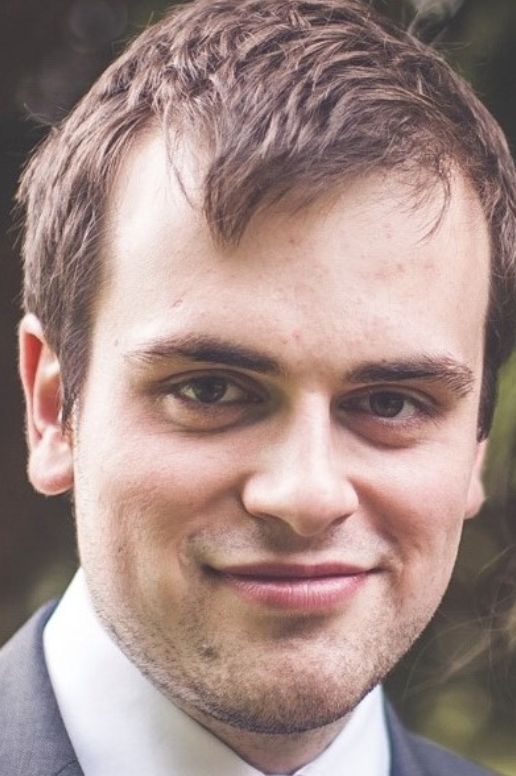
\includegraphics[width=0.5\linewidth]{matt.png}

    \vspace{0.15cm}

    {\scriptsize
    \begin{minipage}{0.9\linewidth}
    \centering
    Reference: M. J. Colbrook. \emph{Infinite-Dimensional Spectral Computations: Foundations, Algorithms, and Modern Applications}. Cambridge University Press, 2026. Forthcoming.
    \end{minipage}
    }
\end{center}
\end{column}

\end{columns}

\end{frame}




\begin{frame}[t]{The Algorithm}

% Step title area
\begin{overlayarea}{\textwidth}{0.10\textheight}
\centering
\only<1>{}
\only<2>{\Large 1. Discretize the complex plane}
\only<3>{\Large 2. Solve auxiliary eigenproblems}
\only<4>{\Large 3. Construct the approximation}
\end{overlayarea}

\vspace{-0.5em}

% Fixed diagram area
\begin{overlayarea}{\textwidth}{0.50\textheight}
\begin{center}

%====================================================
% Overlays 1--3
%====================================================
\only<1-3>{
\tikzset{
    axis/.style={thick, gray!70, -{Latex[length=2mm]}},
    specpt/.style={circle, fill=red!80!black, inner sep=1.7pt},
    gridpt/.style={circle, fill=black!55, inner sep=1.2pt},
    testpt/.style={circle, fill=green!60!black, draw=green!50!black, inner sep=2pt},
    disc/.style={dashed, gray!70, thick},
    lab/.style={font=\small}
}

\begin{tikzpicture}[xscale=0.9, yscale=0.9]

% Fixed bounding box
\path[use as bounding box] (-2.3,-2.1) rectangle (2.3,2.25);

\colorlet{annotblue}{blue}

% axes
\draw[axis] (-2,0) -- (2.2,0);
\draw[axis] (0,-2) -- (0,2.2);

% grid points and computational disc appear on overlay 2 onward
\only<2->{
    \foreach \x in {-1.2,-0.6,0,0.6,1.2}{
        \foreach \y in {-1.2,-0.6,0,0.6,1.2}{
            \pgfmathsetmacro{\r}{\x*\x+\y*\y}
            \ifdim \r pt < 2.41pt
                \node[gridpt] at (\x,\y) {};
            \fi
        }
    }
    \draw[disc] (0,0) circle (1.55);
}

% isolated spectral points
\node[specpt] at (-1.05,1.15) {};
\node[specpt] at (-1.20,0.75) {};
\node[specpt] at (-0.72,0.86) {};

% continuous spectral curve
\draw[red!80!black, thick]
    (-0.45,-1.35)
    .. controls (-0.30,-0.70) and (0.20,-0.55) ..
    (0.75,-0.45)
    .. controls (1.10,-0.40) and (1.10,-0.15) ..
    (1.35,0.18);

% spectrum label: only appears on overlay 1
\node<1>[
    text=red!80!black,
    font=\small,
    anchor=east
] at (-1.35,-0.95) {$\operatorname{Sp}(A)$};

% grid label: only appears on overlay 2
\node<2>[black!55] at (1.05,1.82) {$\operatorname{Grid}(n)$};

% overlay 3: selected z
\coordinate (zstep) at (0.6,0.6);

\node<3>[testpt] at (zstep) {};
\node<3>[lab, below left=1pt, text=green!50!black] at (zstep) {$z$};

\node<3>[
    overlay,
    align=left,
    text=green!50!black,
    anchor=west,
    font=\small
] (ann) at (1.85,1.25)
{Compute \\ $\Phi_n(z,A)$ and $d_{n,z}$.};

\draw<3>[overlay, ->, green!60!black, thick]
    (ann.west) to[out=200,in=25] ($(zstep)+(0.08,0.03)$);

\end{tikzpicture}
}

%====================================================
% Overlay 4: construct approximation
%====================================================
\only<4>{
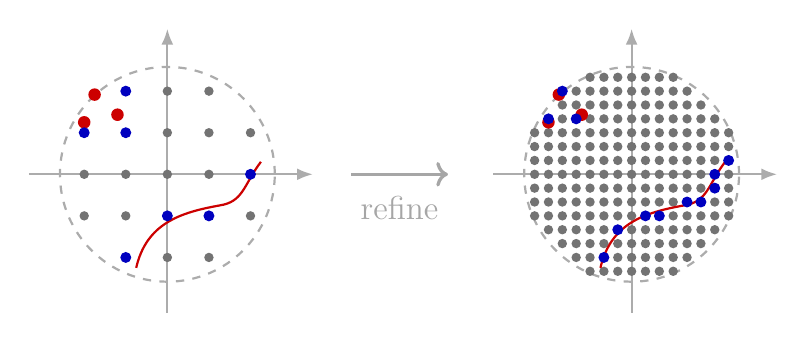
\begin{tikzpicture}[scale=0.88]

\tikzset{
    axis/.style={thick, gray!65, -{Latex[length=2mm]}},
    gridpt/.style={circle, fill=black!55, inner sep=1.2pt},
    approxpt/.style={circle, fill=blue!75!black, inner sep=1.4pt},
    specpt/.style={circle, fill=red!80!black, inner sep=1.6pt},
    disc/.style={dashed, gray!65, thick}
}

%====================================================
% LEFT: coarse grid
%====================================================
\begin{scope}[shift={(-3.35,0.15)}]

    \def\R{1.55}
    \def\h{0.60}

    % disc and axes
    \draw[disc] (0,0) circle (\R);
    \draw[axis] (-2.0,0) -- (2.1,0);
    \draw[axis] (0,-2.0) -- (0,2.1);

    % coarse uniform grid in the disc
    % \foreach \i in {-2,-1,...,2}{
    %     \foreach \j in {-2,-1,...,2}{
    %         \pgfmathsetmacro{\x}{\i*\h}
    %         \pgfmathsetmacro{\y}{\j*\h}
    %         \pgfmathsetmacro{\rsq}{\x*\x+\y*\y}
    %         \ifdim \rsq pt < 2.41pt
    %             \node[gridpt] at (\x,\y) {};
    %         \fi
    %     }
    % }

    {
    \foreach \x in {-1.2,-0.6,0,0.6,1.2}{
        \foreach \y in {-1.2,-0.6,0,0.6,1.2}{
            \pgfmathsetmacro{\r}{\x*\x+\y*\y}
            \ifdim \r pt < 2.41pt
                \node[gridpt] at (\x,\y) {};
            \fi
        }
    }
    }

    % isolated spectral points
    \node[specpt] at (-1.05,1.15) {};
    \node[specpt] at (-1.20,0.75) {};
    \node[specpt] at (-0.72,0.86) {};

    % continuous spectral curve
    \draw[red!80!black, thick]
        (-0.45,-1.35)
        .. controls (-0.30,-0.70) and (0.20,-0.55) ..
        (0.75,-0.45)
        .. controls (1.10,-0.40) and (1.10,-0.15) ..
        (1.35,0.18);

    % selected coarse-grid points
    \foreach \p in {
        (-1.2,0.6),
        (-0.6,1.2),
        (-0.6,0.6),
        (-0.6,-1.2),
        (0,-0.6),
        (0.6,-0.6),
        (1.2,0)
    }{
        \node[approxpt] at \p {};
    }

\end{scope}

%====================================================
% ARROW
%====================================================
\draw[->, very thick, gray!70] (-0.70,0.15) -- (0.70,0.15)
node[midway, below=4pt, text=gray!70] {\large refine};

% \node[blue!75!black, font=\footnotesize] at (0,-1.55)
%     {blue points: approximate spectrum};

%====================================================
% RIGHT: refined grid
%====================================================
\begin{scope}[shift={(3.35,0.15)}]

    \def\R{1.55}
    \def\h{0.20}

    % disc and axes
    \draw[disc] (0,0) circle (\R);
    \draw[axis] (-2.0,0) -- (2.1,0);
    \draw[axis] (0,-2.0) -- (0,2.1);

    % refined uniform grid in the disc
    \foreach \i in {-7,-6,...,7}{
        \foreach \j in {-7,-6,...,7}{
            \pgfmathsetmacro{\x}{\i*\h}
            \pgfmathsetmacro{\y}{\j*\h}
            \pgfmathsetmacro{\rsq}{\x*\x+\y*\y}
            \ifdim \rsq pt < 2.4026pt
                \node[gridpt] at (\x,\y) {};
            \fi
        }
    }

    % isolated spectral points
    \node[specpt] at (-1.05,1.15) {};
    \node[specpt] at (-1.20,0.75) {};
    \node[specpt] at (-0.72,0.86) {};

    % continuous spectral curve
    \draw[red!80!black, thick]
        (-0.45,-1.35)
        .. controls (-0.30,-0.70) and (0.20,-0.55) ..
        (0.75,-0.45)
        .. controls (1.10,-0.40) and (1.10,-0.15) ..
        (1.35,0.18);

    % selected refined-grid points
    \foreach \p in {
        (-1.2,0.8),
        (-1.0,1.2),
        (-0.8,0.8),
        (-0.4,-1.2),
        (-0.2,-0.8),
        (0.2,-0.6),
        (0.4,-0.6),
        (0.8,-0.4),
        (1.0,-0.4),
        (1.2,-0.2),
        (1.2,0.0),
        (1.4,0.2)
    }{
        \node[approxpt] at \p {};
    }

\end{scope}

\end{tikzpicture}
}

\end{center}
\end{overlayarea}
\vspace{-0.8em}

% Fixed explanation area
\begin{overlayarea}{\textwidth}{0.18\textheight}

\only<1>{
% intentionally blank: spectrum only
}

\only<2>{
\vspace{1em}
\begin{itemize}
    \item To approximate $\operatorname{Sp}(A)$, discretize the complex plane with a uniform grid covering a disc of radius $n$, denoted $\operatorname{Grid}(n)$.
\end{itemize}
}

\only<3>{
\begin{itemize}
    \item For each $z \in \operatorname{Grid}(n),$ compute an approximation $\Phi_n(z,A) \approx \gamma(z,A)$ and the associated bound on the distance to the spectrum, $d_{n,z}.$
    \item This often requires approximating the smallest eigenvalue of the $n$-dimensional discretizations of $(A-zI)^*(A-zI)$ and $(A-zI)(A-zI)^*.$
\end{itemize}
}

\only<4>{
\vspace{1em}
\begin{itemize}
    \item Using the computed information, approximate $\text{Sp}(A)$ by the subset of grid points that are sufficiently close to the spectrum. These points are shown in blue.
\end{itemize}
}

\end{overlayarea}

\end{frame}

\begin{frame}{Motivating Challenges}
    \only<1->{
\begin{specbox}{green!45!black}{The Success of Colbrook's Algorithm}
Under certain conditions on $A,$ Colbrook's algorithm yields a convergent approximation of $\text{Sp}(A)$ that captures the continuous components of the spectrum and does not suffer from spectral pollution or spectral invisibility.
\end{specbox} 
}

\only<2->{
\vspace{0.3em}

\begin{specbox}{red}{Motivating Challenges}
\begin{enumerate}
    \item To compute $d_{n,z}$ we solve eigenproblems at each $z \in \text{Grid}(n).$ This is expensive.
    \vspace{0.5em}
    \item If the discretization of an eigenproblem is too coarse, $d_{n,z}$ does not tightly bound $\text{dist}(z, \text{Sp}(A)).$ 
\end{enumerate}
\end{specbox}
}
\end{frame}

\begin{frame}{Project Motivation}
\only<1->{
\begin{specbox}{blue}{Guiding Question}
    How can we exploit the structure of the auxiliary eigenproblems in Colbrook's algorithm to solve them efficiently? 
\end{specbox}
}
\vspace{1em}
\only<2->{
\begin{specbox}{blue}{Follow-Up Questions}
    \begin{enumerate}
        \item Can \textbf{multilevel methods} be used to reduce the cost of solving the eigenproblem associated with each \(z \in \operatorname{Grid}(n)\)?
        % Can we effectively combine Colbrook's algorithm with \textbf{multilevel methods} for eigenproblems to try and ease the computational effort of solving an eigenproblem at each $z \in \text{Grid}(n)?$
        \vspace{0.25em}
        \item Can \textbf{goal-based adaptivity} be used to compute bounds on \(\operatorname{dist}(z,\operatorname{Sp}(A))\) to some desired accuracy?
        % Can we effectively combine Colbrook's algorithm with \textbf{goal-based adaptivity} to compute a bound on $\text{dist}(z, \text{Sp}(A))$ to some desired accuracy?
    \end{enumerate}
\end{specbox}
}


\end{frame}

\begin{frame}[t]{Project Roadmap}

\vspace{-0.4em}

\begin{center}
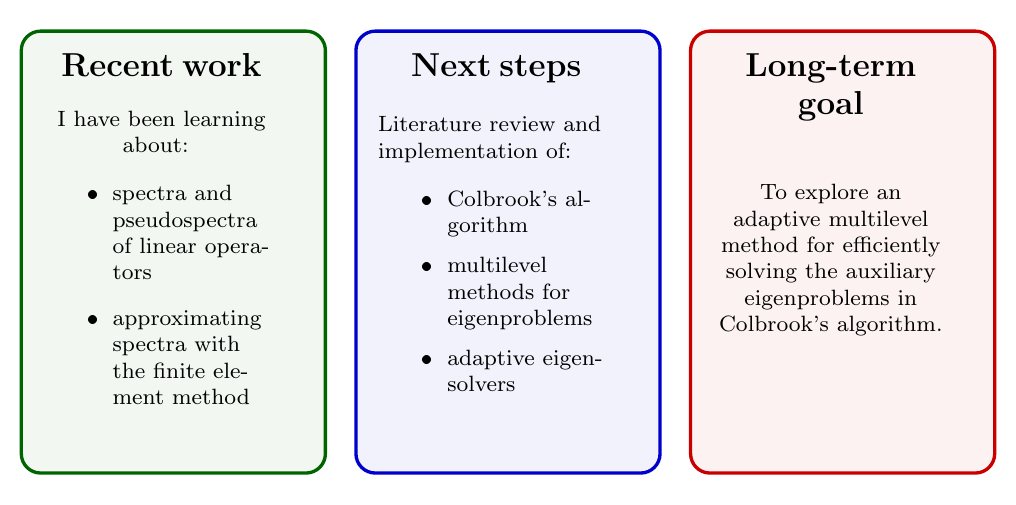
\begin{tikzpicture}[
    >=Latex,
    every node/.style={font=\footnotesize},
    phasebox/.style={
        rounded corners=7pt,
        very thick,
        text width=3.3cm,
        align=left,
        inner sep=8pt
    },
    arrow/.style={
        very thick,
        black,
        -{Latex[length=2.2mm]},
        shorten <=2pt,
        shorten >=2pt
    }
]

\path[use as bounding box] (-6.1,-2.85) rectangle (6.1,2.85);

%------------------------------------------------
% Box 1
%------------------------------------------------
\node<1->[
    phasebox,
draw=RoadGreen,
fill=RoadGreen!5
] (box1) at (-4.25,0) {
\begin{minipage}[t][5.05cm][t]{3cm}
    \centering
    {\large\bfseries Recent work\par}

    \vspace{1em}

    I have been learning about:
    \vspace{0.35em}

    \RaggedRight
    \begin{itemize}\itemsep0.6em
    
        \item spectra and pseudospectra of linear operators
        \item approximating spectra with the finite element method
    \end{itemize}
\end{minipage}
};

%------------------------------------------------
% Box 2
%------------------------------------------------
\node<2->[
    phasebox,
draw=RoadBlue,
fill=RoadBlue!5
] (box2) at (0,0) {
\begin{minipage}[t][5.05cm][t]{3cm}
    \centering
    {\large\bfseries Next steps\par}

    \vspace{1.25em}

    \RaggedRight
    Literature review and implementation of:

    \vspace{0.35em}

    \begin{itemize}\itemsep0.35em
        \item Colbrook's algorithm
        \item multilevel methods for eigenproblems
        \item adaptive eigensolvers
    \end{itemize}
\end{minipage}
};

%------------------------------------------------
% Box 3
%------------------------------------------------
\node<3->[
    phasebox,
draw=RoadRed,
fill=RoadRed!5
] (box3) at (4.25,0) {
\begin{minipage}[t][5.05cm][t]{3cm}
    \centering
    {\large\bfseries Long-term goal\par}

    \vspace{2.5em}

    \Rcentering
    To explore an adaptive multilevel method for efficiently solving the auxiliary eigenproblems in Colbrook's algorithm.
\end{minipage}
};

%------------------------------------------------
% Arrows
%------------------------------------------------
% \draw<2->[arrow] (box1.east) -- (box2.west);
% \draw<3->[arrow] (box2.east) -- (box3.west);

\end{tikzpicture}
\end{center}

\end{frame}




\appendix 

\begin{frame}{Extra: The Spectra of the Shift Operators}
    Consider the $\ell^2$ sequence space. This is a Hilbert space with norm $\| x \|^2 = \sum_{n=1}^{\infty} |x_n|^2$ and inner product $\langle x, y \rangle = \sum_{n=1}^{\infty} x_n \overline{y_n}.$

    \vspace{1em}

    Define the left and right shift operators on $\ell^2$ as 
    $$ L(x_1, x_2, \dots) = (x_2, x_3, \dots) \,\, \text{ and } \,\, R(x_1, x_2, \dots) = (0, x_1, x_2, \dots),$$
    respectively.

    \vspace{1em}
     
    Notice that $L^* = R$ and $\| R \| = \|L\| = 1.$

    \vspace{1em}

        When $A$ is bounded,
     $\text{Sp}(A) \subset \{ z \in \mathbb{C} \mid |z| \le \|A\| \}.$
    Thus,
     $$ \text{Sp}(L),  \text{Sp}(R) \subset \{ z \in \mathbb{C} \mid |z| \le 1 \}.$$
    
\end{frame}

% \begin{frame}{Continued: The Spectra of the Shift Operators}

%     When $A$ is bounded,
%     $$ \text{Sp}(A) \subset \{ z \in \mathbb{C} \mid |z| \le \|A\| \}.$$

%     Since $\|L \| = \|R\| = 1,$
%     $$ \text{Sp}(L) \subset \{ z \in \mathbb{C} \mid |z| \le 1 \}$$
%     and 
%     $$ \text{Sp}(R) \subset \{ z \in \mathbb{C} \mid |z| \le 1 \}.$$

% \end{frame}

\begin{frame}{Continued: The Spectra of the Shift Operators}

    The eigenvalues of $L$ are found by solving $Lx = \lambda x$ for any $\lambda \in \mathbb{C}$ and a nonzero $x \in \ell^2.$

     \vspace{0.5em}

    Thus, the eigenvectors are of the form
    $$ x = x_1 (1, \lambda, \lambda^2, \dots)$$
    and must satisfy
    $$ |x_1|^2 \sum_{n=0}^{\infty} |\lambda|^{2n} < \infty.$$


 From this we find that
    $$\Gamma(L) = \text{set of eigenvalues of } L = \{ \lambda \in \mathbb{C} \mid |\lambda| < 1 \} \subset \text{Sp}(L).$$

     \vspace{0.5em}

    Since the spectrum of a bounded operator is closed, the closed disk must also be in $\text{Sp}(L).$ Thus,  $ \text{Sp}(L) \supset \{ z \in \mathbb{C} \mid |z| \le 1 \},$  $ \text{Sp}(L) \subset \{ z \in \mathbb{C} \mid |z| \le 1 \},$ and so
     $$ \text{Sp}(L) = \{ z \in \mathbb{C} \mid |z| \le 1 \}.$$

\end{frame}

\begin{frame}{Continued: The Spectra of the Shift Operators}

    The eigenvalues of $R$ are found by solving $Rx = \lambda x$ for any $\lambda \in \mathbb{C}$ and a nonzero $x \in \ell^2.$
     \vspace{1em}
     
    In doing so we find that the eigenvectors must satisfy
    $$ (0, x_1, x_2, \dots) = \lambda(x_1, x_2, \dots).$$ 
    % Equivalently,
    % $$ \lambda x_1 = 0, \,\, \lambda x_2 = x_1, \,\, .\dots$$
   The only solution is $x=0$ which cannot be an eigenvector. Thus, $R$ has no eigenvalues.

     \vspace{1em}

    When $A$ is closed and densely defined, $\text{Sp}(A^*) = \{\overline{z} \mid z \in \text{Sp}(A) \}.$ Here, $L$ and $R$ are bounded operators on all of $\ell^2$ and $L^* = R$. Thus, 
    $$ \text{Sp}(R) = \{\overline{z} \mid z \in \text{Sp}(L) \} = \{ z \in \mathbb{C} \mid |z| \le 1 \}.$$



\end{frame}



\end{document}
